%\documentclass[xcolor=svgnames]{beamer}
%\includeonlyframes{current}


\documentclass[xcolor=svgnames]{beamer}

\usepackage{MnSymbol,wasysym}
\usepackage[utf8]    {inputenc}
\usepackage[T1]      {fontenc}
\usepackage[english] {babel}
\usepackage{upquote} 
\usepackage{amsmath,amsfonts,graphicx}
\usepackage{beamerleanprogress}
\usepackage{xcolor}
\usepackage{soul}
%\usepackage{verbatim}
\usepackage{multicol}
\usepackage{tikz} 
\usepackage[export]{adjustbox}
\usepackage{verbatim}

\definecolor{iyellow}{RGB}{255, 162, 23}
\definecolor{sgreen}{RGB}{118, 191, 138}

\newcommand{\yellow}[1]{\textcolor{iyellow}{#1}}
\newcommand{\orange}[1]{\textcolor{OrangeRed}{#1}}
\newcommand{\green}[1]{\textcolor{sgreen}{#1}}
\newcommand{\red}[1]{\textcolor{red}{#1}}
\newcommand{\blue}[1]{{\textcolor{blue}{#1}}}
%\newcommand{\newpt}{\par \vspace{5mm}}

\newcommand{\cell}[1]{{\sf \textbf{\textcolor{DarkMagenta}{#1}}}}
\newcommand{\ft}[1]{\frametitle{#1}}
\newcommand{\ra}{$\rightarrow$ }
\newcommand{\eol}{\\[1em]}
\newcommand{\btVFill}{\vskip0pt plus 1filll}

\newcommand{\define}[1]{\textbf{\textcolor{orange}{#1}}}
\newcommand{\answer}[1]{\textit{\textbf{\textcolor{iyellow}{#1}}}}
\newcommand{\command}[1]{\texttt{\textbf{\textcolor{DarkMagenta}{#1}}}}


\usepackage{hyperref}
\hypersetup{
    colorlinks=true,
    linkcolor=blue,
    filecolor=magenta,      
    urlcolor=cyan,
}

\usepackage{fancyvrb}
\usepackage[T1]{fontenc}
\usepackage[utf8]{inputenc}
\usepackage{tikz}
\usetikzlibrary{shadows}

\newcommand*\keystroke[1]{%
  \tikz[baseline=(key.base)]
    \node[%
      draw,
      fill=white,
      drop shadow={shadow xshift=0.25ex,shadow yshift=-0.25ex,fill=black,opacity=0.75},
      rectangle,
      rounded corners=2pt,
      inner sep=1pt,
      line width=0.5pt,
      font=\scriptsize\sffamily
    ](key) {#1\strut}
  ;
}

\title
  [Data 301 Data Analytics\hspace{2em}]
  {Data 301 Data Analytics\\
Microsoft Execl VBA\\
Excel Part 3 of 3}

\author
  [Dr.\ Irene Vrbik]
  {Dr.\ Irene Vrbik}

\date
  {}

\institute
  {University of British Columbia Okanagan \newline irene.vrbik@ubc.ca}


\graphicspath{{img/}}

\begin{document}

\maketitle

\setbeamersize{description width=0.57cm} % to have less indent with the description environment

\section{Creating Macros}


\frame{
\ft{What is VBA?}

Excel %Visual Basic for Applications (VBA)
Visual Basic for Applications (VBA) is a programming language developed by Microsoft.\eol

It allows users to build their own functions, automate tasks in  several Microsoft applications, including Microsoft Office, and develop customized code.\eol

The language has been part of almost all versions of Office for over 20 years.\eol

VBA allows for expanding the capabilities of Excel and provides a level of customization, eg. adding user-interface elements (buttons, lists) to your spreadsheet.

}

\begin{frame}
  {Why Microsoft Excel Visual Basic for Applications?}
Microsoft Excel VBA allows for automating tasks in Excel and provides a full programming environment for data analysis. 
\begin{itemize}
\item We can use VBA to automate tedious processes in Excel, eg. formatting a month report, creating headers to look a certain way, ... \eol
\end{itemize}

Excel VBA is commonly used in high finance (eg. investment banking) and frequency trading applications for creating and validating financial models.\eol

Using Excel VBA will be our first practice with programming and allow us to explore fundamental programming concepts of commands, variables, decisions, repetition, objects, and events.
\end{frame}

\frame{
\ft{Macros}
A \emph{macro} (short for macroinstruction) is a recorded set of actions that is saved so that they can be easily executed again.\eol

If you do the same set of actions repetitively, then creating a macro allows for doing all those actions with one command.\eol
Macros are accessible either under the {\bf View} or the  {\bf Developer} tab in the Ribbon (I usual navigate to the latter).\eol

Macros are converted into VBA \emph{programs}; that is, a sequence of instructions that a computer can interpret and execute.  
}
%A macro (short for "macroinstruction", from Greek ?????? 'long') in computer science is a rule or pattern that specifies how a certain input sequence (often a sequence of characters) should be mapped to a replacement output sequence (also often a sequence of characters) according to a defined procedure. The mapping process that instantiates (transforms) a macro use into a specific sequence is known as macro expansion. 

\frame{
\ft{Developer Tab}
The Developer tab contains icons for performing VBA and macro development.  \eol

This tab is disabled by default.\eol

To add the Development tab on a PC, go to {\bf File}, {\bf Options}, {\bf Customize Ribbon} and make sure it is checked beside Developer.\eol

For a Mac, go to {\bf Excel}, {\bf Preferences}, {\bf View}.  Under the  \textit{In Ribbon, Show} heading, select the checkbox marked ``Developer Tab"

}

\frame[label=current]{
\ft{Recording a Macro }



To record a macro, go to the {\bf View} tab or {\bf Developer} tab and select  the ``Record Macro'' button  $\vcenter{\hbox{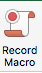
\includegraphics[width=2em]{img/recordmacro.png}}}$
  
  \begin{center}
     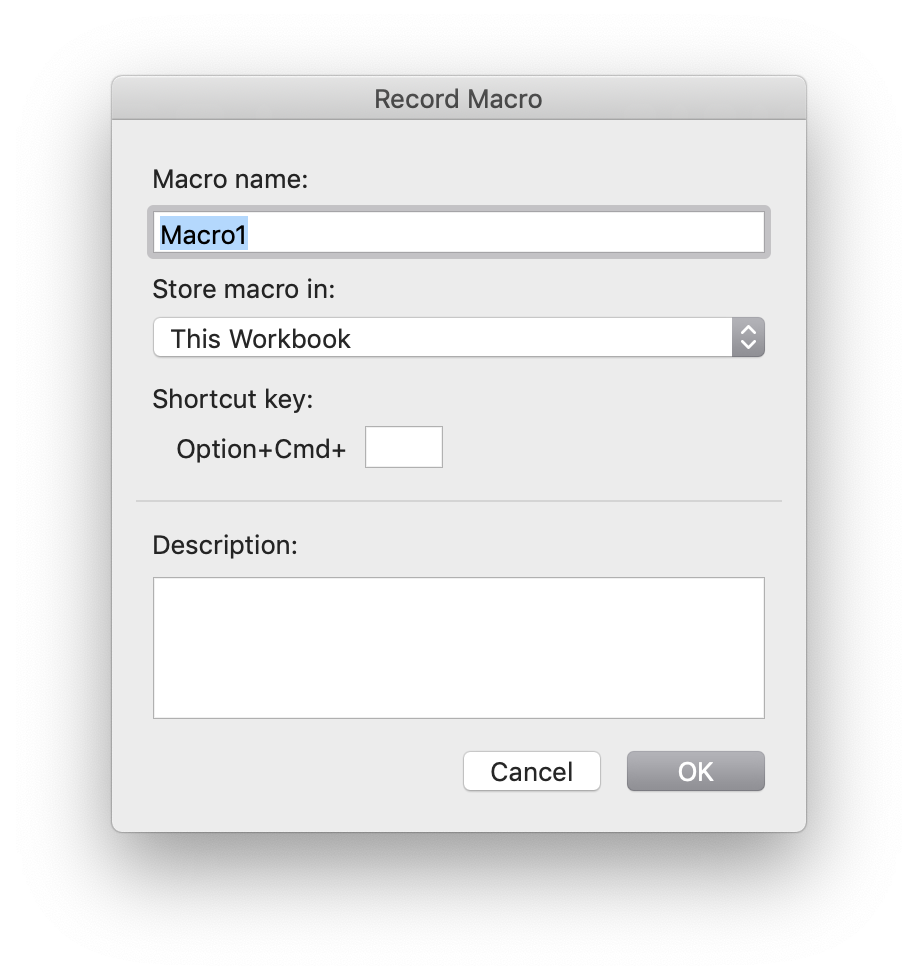
\includegraphics[width=0.4\textwidth]{img/recordMac}
%    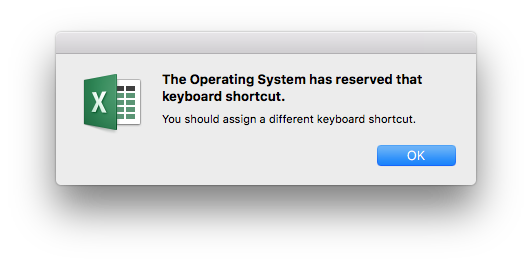
\includegraphics[width=0.4\textwidth]{img/ReservedShortcut}
  \end{center}
  \vspace{-1em}
  Once selected, pop-up window will appear prompting you to enter a Macro name and (optional) keyboard shortcut.\eol
  
  
}
  
  \frame[label=current]{
\ft{Recording a Macro }

{Macro names cannot contain spaces or begin with a number.}\eol
{When possible, you should try to give a meaningful/concise macro name that provides some insight into what it does.}\eol
{It is recommended to use \keystroke{Ctrl}+\keystroke{Shift}+{\tt <Key>} (PC)/\keystroke{Option}+\keystroke{Cmd}+{\tt <Key>} (Mac) for a Shortcut key so that you do not override built-in shortcuts.}\eol
{Macs will give you a warning when you attempt to override an existing shortcut.}\eol
{A macro can be created without assigning it a shortcut key.}

} 


  \frame[label=current]{
\ft{Recording a Macro }
\begin{itemize}
 \item To record your macro's actions, fill out the fields in the pop-up window, click OK then perform the actions you wish to record.

 \item Once you start, the {\bf Record Macro} 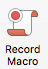
\includegraphics[width=2.5em]{img/recmac.png} will become 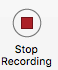
\includegraphics[width=2.5em]{img/stopmac.png}, a {\bf Stop Recording} button   \medskip
\item Save for cursor movements, Excel will record your every action until you select the {\bf Stop Recording} button.
 \medskip
 \item Next time we would like to perform these actions, rather than going through all the motions, we can simply run this recorded macro.
\end{itemize}
} 



\begin{frame}
\begin{columns}[T] % align columns
\begin{column}{.3\textwidth}
$$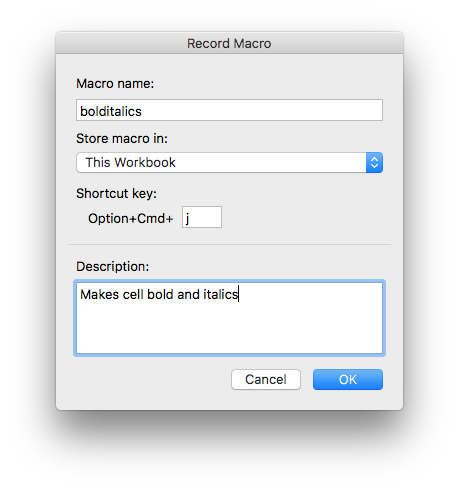
\includegraphics[width=1.5\textwidth]{img/bolditalics}$$
\end{column}%
\hfill%
\begin{column}{.7\textwidth}
\begin{itemize}
%\item Note: Cursor movement is not captured.
\item As a simple example, we could create a macro that bold and italicizes a cell.
\begin{itemize}
\item Macro name: {\tt bolditalics} 
\item Shortcut: Option + Cmd + j
\item Makes cells bold and italics
\end{itemize}
\item While the macro name is pretty self-explanatory, it is usually a good idea to provide a description about what your macro  does.
\end{itemize}
\end{column}%
\end{columns}
\end{frame}



\frame{
\ft{Recording Macros}
By default, macros are created using absolute references %({\tt $A$1} rather than {\tt A1}
\begin{itemize}
\item To use Relative references, we need to turn on the ``Use Relative References" button, \underline{before} we record.\footnote{feature \href{https://answers.microsoft.com/en-us/mac/forum/macoffice2016-macexcel/record-macros-with-relative-references-in-office/8098f458-66b3-4546-a4f2-9b9bb8492c6b}{not available for Macs}}
\item If you want your macro to run on the active cell, make sure we don't move out of the active cell once we start to record our macro.
\end{itemize}
While the Macro Recorder makes creating macros very easy, it has it's limitations:
\begin{itemize}
%\item \alert{\frownie{}\frownie{} There is no way (that I can find) to do this on a Mac \frownie{}\frownie{}}
\item eg. cannot handle ``loops" (more on loops later)
\item generates more code than is necessary (which can slow down your process).

\end{itemize}
%For that reason, we better learn some code \dots
}




\section{Using Macros}

\frame{
\ft{Using a Macro}
There are a number of ways you can use your macro:
\begin{enumerate}
\item With the shortcut key if defined
\item Under the {\bf View} tab, Select {\bf View Macros} (or  {\bf Macros} under the  {\bf Developer} tab)  then highlight the macro name and click {\bf Run}.
\item Assign a macro to a button or on the toolbar.
\end{enumerate}
}

\frame[t]{
\ft{Macro Buttons}
To assign a macro button:
\begin{enumerate}

\item Select the {\bf Developer} tab and click 
$$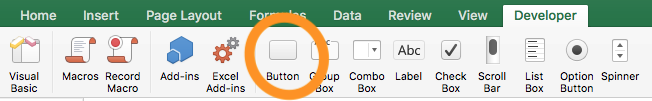
\includegraphics[height=3.5em]{img/button.png}.$$
\item To prompt the Assign Macro popup window, click where you would like this button to appear on your worksheet.
%\item Assign a macro to the button by selecting one from the list of existing macros or creating a brand new one and click OK.
%\item To specify the control properties of the button, right-click it, and then select Format Control....
\end{enumerate}
\btVFill
\textit{{\bf Side-note:} You can also assign macros to shapes ({\bf Insert} "Shapes"), by right-clicking on it, and selecting {\bf Assign Macro}.}
}



\begin{frame}[fragile]
\ft{Macro Buttons}
\begin{enumerate}[3.]
\item Then, either:
\begin{itemize}
\item select the name of an existing macro from those listed in the pop-up window, 
\item press the {\bf Record...} button to record a new macro, or  
\item press {\bf New} to open the VBA editor (more on this later).
\end{itemize}
\begin{center}
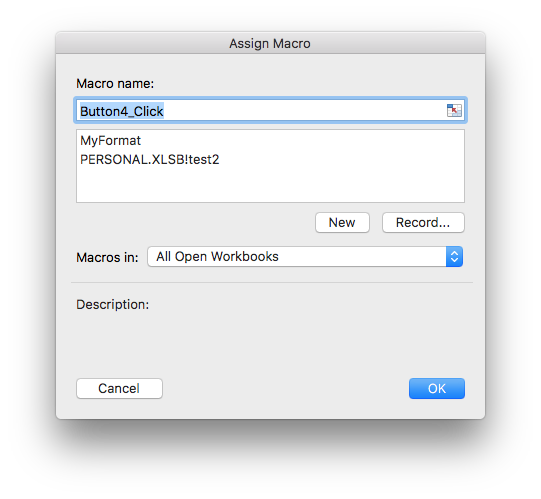
\includegraphics[width=0.7\textwidth]{img/assignMacro.png}
\end{center}

%"New" and the VBA editor will open. Type the name of the macros you wish to assign in the body of the Sub.
%\begin{verbatim}
%  Sub ButtonX_Click() 
%      bolditalics
%      undercenter
%  End Sub
%\end{verbatim}
\end{enumerate}
\end{frame}


%
%\frame{
%\ft{Macro Toolbars}
%To add a macro to The Quick Access Toolbar, select:
%\begin{enumerate}
%\item \begin{description}
%\item[PC] {\bf File} \ra {\bf Options} \ra \textit{Quick Access Toolbar}.
%\item[Mac] {\bf Excel} \ra {\bf Preferences} and click \textit{Ribbon and Toolbar} \ra \textit{Quick Access Toolbar} header
%\end{description}
%\item In the ``Choose commands" drop-down menu, select {\bf Macros}
%\item Select the macro and add to your toolbar (click this 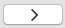
\includegraphics[width=2em]{img/add.png})
%\item  Modify the button with a unique icon (eg. \smiley{})\footnote{This is only available for Windows. Read more \href{https://support.office.com/en-us/article/assign-a-macro-to-a-button-728c83ec-61d0-40bd-b6ba-927f84eb5d2c\#OfficeVersion=Windows}{here}}.
%%\begin{itemize}
%%\item \frownie{}\frownie{} Feature not available on a mac? \frownie{}\frownie{}
%%\end{itemize}
%\end{enumerate}
%There will now be a new shortcut located at the Toolbar above the Ribbon:
%\begin{center}
%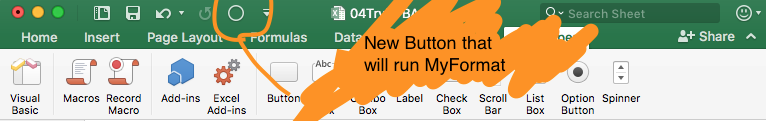
\includegraphics[width=0.9\textwidth]{img/QuickToolbar.png}
%\end{center}
%}
%

\begin{frame}
\ft{Try It: Macros}
\begin{exampleblock}{Question}
Create a macro called {\tt MyFormat} that does the following tasks:
\begin{enumerate}
\item Use a shortcut of \keystroke{Ctrl}+\keystroke{Shift}+\keystroke{b} (PC)/\keystroke{Opt}+\keystroke{Cmd}+\keystroke{b} (Mac).
\item Bolds the cell and makes the font Courier 20
\item Sets the cell background to orange.
\item Centers the text in the cell.
\item Add it to a button in the shape of a star that says OC20
\end{enumerate}
\end{exampleblock}
Try-out your macro using 1) the shortcut key, 2) the macro dialog, and 3) the macro button.
\end{frame}



\begin{frame}{Warning}
\begin{itemize}
\vfill
\item There is no easy way to undo a macro update.
\vfill
\item That is to say, the safety net that comes in the from of the \keystroke{Ctrl}/\keystroke{Cmnd} (Windows/Mac) + \keystroke{Z} keyboard combination will not allow you to undo any changes that your macro made to your document (in fact, running a macro completely erases the Undo list)
\vfill
\item While there is no  intrinsic way of  preserving the Undo list, you can save your workbook immediately before running the macro.  If you want to undo the effects, simply close the workbook without saving and re-open your preserved pre-macro version.
\vfill

\end{itemize}

\end{frame}



\section{Saving}
\frame{
\ft{Saving macros}
In order to save the workbook with the macros we've created while it was open, we need  use a  "macro-enabled" file format.\eol
When you go to save a workbook containing macros, you will receive the following popup
$$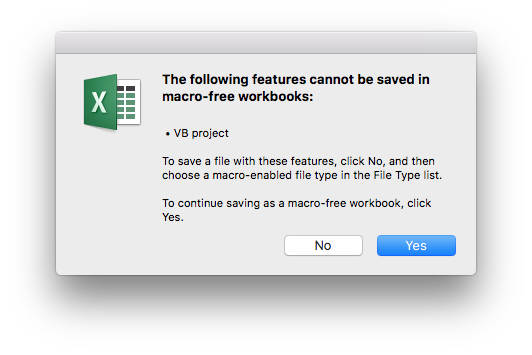
\includegraphics[width=0.5\textwidth]{img/SavingMacro.png}$$
\vspace{-2em}
\begin{itemize}
\item  `Yes' will save it as as macro-free workbook (*.xlsx file)
\item Select `No'  to save it as as macro-enabled workbook (*.xlsm file)
\end{itemize}

}

\frame{
\ft{Saving macros}
Saving a macros to a  given workbook will only allow you to use it with that file.\eol
We could alternatively save it to a \emph{Personal Workbook} allowing them to be used in multiple workbooks.\eol
Your Personal Workbook is a hidden workbook saved under the name {\bf personal.xlsb}\eol
This file loads every time you open up Excel. \eol
Hence saving a macro to {\bf personal.xlsb} will allow you to use that macro on any workbook that you open on your computer
}


\frame{
\ft{Saving macros}
To save it to your personal workbook,  select the "Personal Macro Workbook" option in the drop-down menu for "Store Macro in"
$$
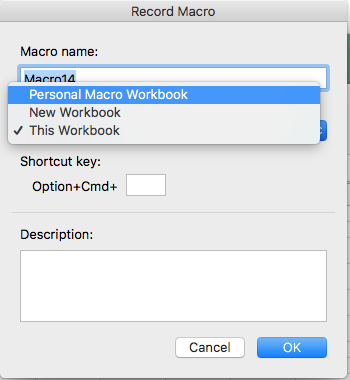
\includegraphics[width=0.4\textwidth]{img/PWB.png}$$
}


\frame{
\ft{Macro Security}
Since macros can execute any code, they have been a target for virus writers.  \eol
Understanding the source of the Excel spreadsheet that contains macros is important when deciding to run them or not.\eol

Excel has \emph{macro security settings} to allow you to enable or disable running macros.  \eol

Spreadsheets with macros often will generate a warning when opening them:
$$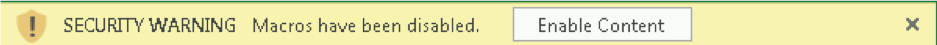
\includegraphics[width=0.9\textwidth]{img/security}$$
}

\frame{
\ft{Macro Security Settings}
The default security is  to \emph{Disable all macros with notification}. This prevents macros from running but displays a warning allowing you to enable them.\eol
One of the biggest issues with macros is security. \alert{Make sure you are only using macros from a trusted source.}\eol

To change these defaults (which I don't recommend):
\begin{description}
\item[Windows]  click "Macro Security" located below the "Record Macro" button on the {\bf Developer} tab
\item[Mac] Navigate to {\bf Excel} in the toolbar \ra {\bf Preference} "Security \& Privacy"
\end{description}
  Select a desired option in Macro Settings category, under the \textit{Macro Security} header.
%\begin{tikzpicture}[remember picture,overlay]%[xshift=65mm,yshift=-48mm,anchor=north west]
%\node at (current page.center) {\includegraphics<handout:0| beamer:1>[width=.7\textwidth]{img/securityPC}};
%\end{tikzpicture}
%\begin{tikzpicture}[remember picture,overlay]%[xshift=65mm,yshift=-48mm,anchor=north west]
%\node at (current page.center) {\includegraphics<handout:0| beamer:2>[width=.7\textwidth]{img/securityOpts}};
%\end{tikzpicture}
}

\frame{
\ft{Macro Security Settings}
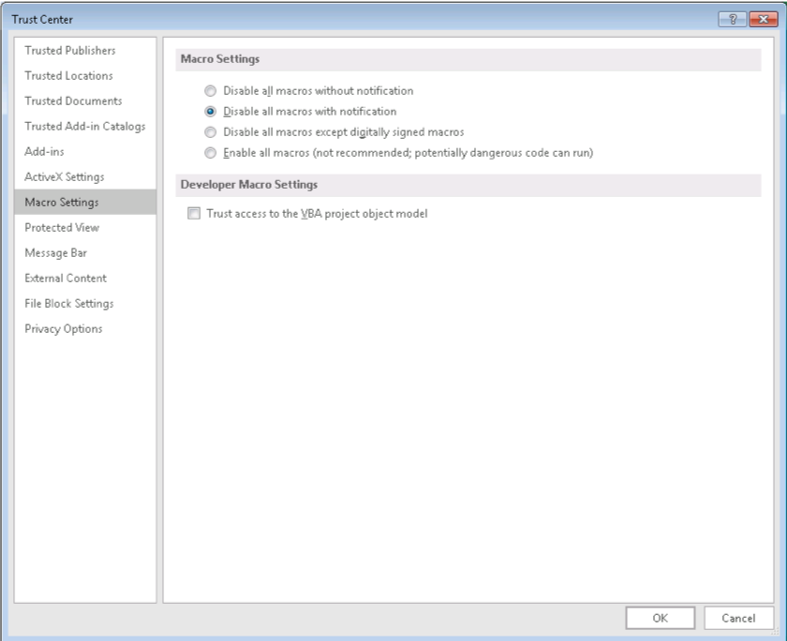
\includegraphics[height=.5\textheight]{img/securityPC}
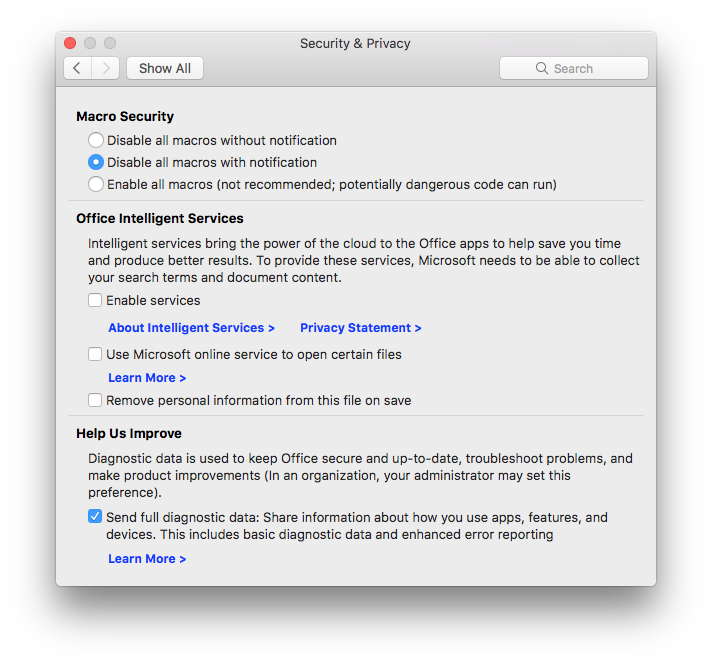
\includegraphics[height=.55\textheight]{img/securityOpts}
}



\frame{
\label{editmacro}
\ft{Macros: Implementation}
Macros are converted to Visual Basic (VB) code.\eol

You can edit macro code and create your own code.\eol

Under the {\bf Developer}  tab, select the  {\bf Macros} button then click the {\bf Edit} button in the pop-up window.  \eol % macro to modify the code.\eol

The code will then open in you \emph{Visual Basic Editor (VBE)}\eol
 {\bf Tip:} It is best practice to break long tasks  into, smaller relevant macros rather than one big macro.\eol
 {\bf Side-note:} Macros can be written for and any other Office application that supports VBA.  

}


\begin{frame}[fragile]{Recording a Macro}
Here is the VBA code that was produced during our {\tt bolditalics} macro recording:
\begin{Verbatim}[xleftmargin=.5in, numbers=left]
Sub bolditalics()
'
' bolditalics Macro
' bold and italicize text
'
' Keyboard Shortcut: Ctrl+j
'
    Selection.Font.Bold = True
    Selection.Font.Italic = True
End Sub
\end{Verbatim}
\end{frame}


\begin{frame}[fragile]\ft{Comments}
\begin{itemize}
\item The apostrophe indicate the starting of a \textit{comment}.  
\medskip
\item \emph{Comments} are ignored by the computer and are used by the programmer to document and explain the code.
\medskip
\item On the previous slide, our comments provide the name of our macro, a description of what it does and the keyboard shortcut information.
\medskip
\item If we were to remove those commented lines (ie. lines 2--7), the macro would still run exactly the same; however, a reader of the VBA code would have a harder time determining what this macro does.
\end{itemize}
\end{frame}



\frame{
\ft{Integrated Development Environment}

An integrated development environment (IDE)  enables programmers to consolidate the different aspects of writing a computer program.\eol

More generally, a IDE provides a convenient way for you to write, compile, and run your code all in one place (as opposed to having to open many applications and windows).\eol

An IDE typically contains a code editor, a compiler or interpreter, and a debugger, accessed through a graphical user interface (GUI). 
\begin{itemize}
\item The user writes and edits source code in the code editor. 
\item The compiler translates the source code into a readable language that is executable for a computer. 
\item And the debugger tests the software to solve any issues or bugs.
\end{itemize}
}

\frame{
\ft{Visual Basic Editor}
Visual Basic Editor (VBE) allows editing visual basic code and is a complete IDE.
\begin{itemize}
\item That is to say, ssers can create and edit macros as well as other Visual Basic code with the editor.\eol
\end{itemize}




To open the VBE either:
\begin{itemize}
\item Edit a macro as explained on  \hyperlink{editmacro}{this} slide
\item Under the {\bf Developer} tab click the {\bf Visual Basic} button 
$$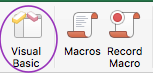
\includegraphics[height=3em]{img/vbButton}$$
\item or use the keyboard shortcut: \keystroke{Alt}+\keystroke{F11}.\eol

\end{itemize}

%There is also a quick button for this in the left hand side of the Developer tab:
%$$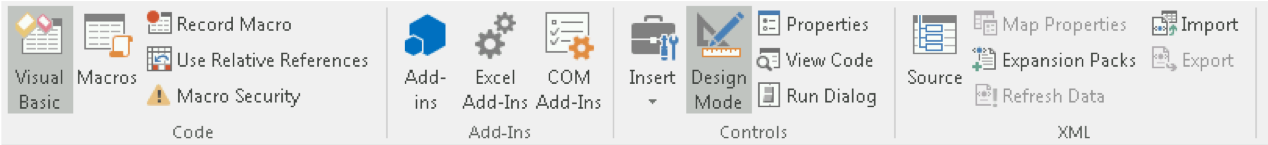
\includegraphics[width=0.8\textwidth]{img/VBE}$$
}

\frame{
\ft{Visual Basic Editor}
$$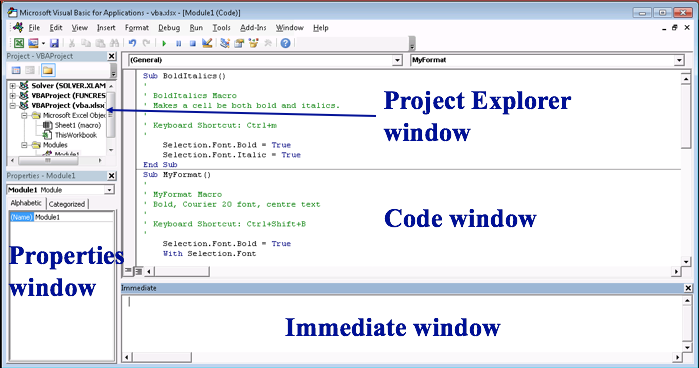
\includegraphics[width=0.9\textwidth]{img/VBEwindow}$$
If you don't see the Immediate window, you can add by going to {\bf View} $>$ Immediate window (while in VBE mode).
}
% https://www.youtube.com/watch?v=NpvvwrdDcQk

\begin{frame}{Visual Basic Editor}
\begin{description}
\item[Project (Explorer) window]  This window shows the tree diagram with every workbook and its worksheets that are currently opened  organizes code files (modules). You can expand and collapse them by clicking the plus and minus signs.
\item[Code window] shows source code for editing.  By default, this windows is empty. Here, you can put your VBA code. In order to open this window double-click one of the objects in the Project window.
\item[Immediate window] allows for execution of commands and getting immediate results.
\item [Properties window] display properties and values of currently selected object.
\end{description}

%http://excel.officetuts.net/en/training/visual-basic-editor-vbe
%Toolbar
\end{frame}

\begin{frame}{Visual Basic Editor - Toolbar}

In the Toolbar, you can find buttons to which you can have quick and easy access.\\
\medskip
For example:
\begin{itemize}
\item    running  a macro (
\includegraphics[width=1em]{img/start.png}) , 
\item stopping  a macro (
\includegraphics[width=1em]{img/stop.png}), 
\item switching back to Excel (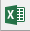
\includegraphics[width=1em]{img/excel.png}) ,
\item  saving the macro (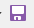
\includegraphics[width=1em]{img/save.png}) 
\item and more \dots
\end{itemize}
%Code window
%
%Immediate window
%This window is useful if you want to debug your code. You can hide it by clicking the �x� button in the upper right corner.
%Properties Window
%As the name suggests it contains a list of properties that define this particular object.

\end{frame}




%https://www.emagenit.com/VBA%20Folder/what_is_a_vba_module.htm
\begin{frame}{Modules}


\begin{minipage}{\textwidth}
\begin{columns}[T]
\begin{column}{0.6\textwidth}
\begin{itemize}
\item A VBA project is a collection of so-called \emph{modules}
\medskip
\item You can think of a VBA module as a text document containing your VBA code.
\end{itemize}
\end{column}
\begin{column}{0.3\textwidth}
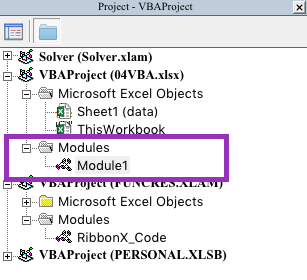
\includegraphics[width=0.98\textwidth]{modules}
\end{column}
\end{columns}
\end{minipage}


\begin{itemize}
\medskip\item All of your code can go into a single module; however, you may choose to save  your code across multiple modules for organizing large projects.
\medskip
\item For more information see \href{https://www.emagenit.com/VBA\%20Folder/what\_is\_a\_vba\_module.htm}{here}
\end{itemize}

\begin{exampleblock}{}{\bf Exercise}: Open the VB Editor in a window beside your active workbook.  Press the record macro button and see how the VBA code produce before you eyes!
\end{exampleblock}

\end{frame}



\begin{frame}{Immediate Window}
\begin{itemize}
\item The VBA Immediate Window is a window from which you can get immediate answers about your Excel files, and quickly execute code. 
\medskip
\item {\bf Tip from \href{https://www.excelcampus.com/vba/vba-immediate-window-excel/}{Excelcampus}} If you would like do ``undock" the immediate window from the VB editor:
\begin{enumerate}
\item Left-click and hold on the top bar of the immediate window.
\item Drag it out of the VB Editor window. The immediate window becomes a free floating window that you can put on top of Excel.
\item To re-dock it, double-click on the top bar of the immediate window. 
\end{enumerate}
\medskip
\item For instance, you can use the Immediate Window for performing simple calculations. For example type {\tt ?765*39} into the Immediate Window and press \keystroke{ENTER}.  The solution {\tt 29835} should appear directly below.
\end{itemize}
\end{frame}


\begin{frame}[fragile]{Visual Basic Editor: Immediate Window}
The {\tt ?} (or alternatively {\tt PRINT} or {\tt Debug.Print}\footnote{use within a VBA program; see Example 4 \href{https://www.excelcampus.com/vba/vba-immediate-window-excel/}{here}}) evaluates/displays specified information to the immediate window.
\begin{itemize}
\item You may  use {\tt msgbox} to  display them in a pop-up window.
%\medskip
%\end{itemize}
%In addition we get  information about the workbook that you currently have open and active in the background.  For example:
%\begin{itemize}
\item {\tt ?Worksheets.Count} prints the number of worksheets in our workbook
\item \verb|? Range("A2").Value| prints the value currently stored in  \cell{A2}  
%\item \verb|?Selection.Interior.ColorIndex| will return the color o
%\item {\tt ActiveCell.Value = 10} changes the value in the active cell
\item \dots
\item See more examples in the {\bf ImmediateWindowExamples} file uploaded to Canvas
\end{itemize}
\end{frame}

% https://www.excelcampus.com/vba/vba-immediate-window-excel/
\begin{frame}[fragile]{Visual Basic Editor: Immediate Window}
We can also \dots
\begin{itemize}
\item  format cells.  Eg, center the text in the ``active" cell (ie. the one currently highlighted in a green border):
\begin{Verbatim}[frame=single]
ActiveCell.HorizontalAlignment = xlCenter
\end{Verbatim}
\vfill

\item reassign the value in cell \cell{A2} to 10 using:
 \begin{Verbatim}[frame=single]
Range("A2").Value = 10
\end{Verbatim}
\vfill

\item run a macro by calling it by name. For example, the following  will apply the corresponding macro to the active cell.
\begin{Verbatim}[frame=single]
MyFormat
\end{Verbatim}
\end{itemize}
\vfill
\end{frame}


\begin{frame}[fragile]{Visual Basic Editor: Immediate Window}
We can also use VBA code for doing things we would normally do with our mouse and keyboard.  For example:
\begin{Verbatim}[frame=single]
Worksheets("forms").Activate
Workbooks("04VBA.xlsx").Worksheets("forms").Activate
\end{Verbatim}
will change the active workbook to {\tt forms} in our {\bf 04VBA.xlsx} workbook (if you don't specify the workbook, it will default to the currently active workbook).
\medskip
We can activate worksheets either by name or number:
\begin{Verbatim}[frame=single]
Worksheets(1).Activate
Worksheets("data").Activate
\end{Verbatim}
 %will change the active worksheet back to {\tt data} (or worksheet 1). 
 Alternatively we can also call the sheet by the Excel object name given in the Project window:
\begin{Verbatim}[frame=single]
Sheet1.Activate
\end{Verbatim}
\end{frame}

\begin{frame}[fragile]{Visual Basic Editor: Immediate Window}
We can select certain cells in a similar manner to how we would in an excel formula.  For example
\begin{itemize}
\item \verb|Range("A6").Activate| is equivalent to clicking on cell \cell{A6} with our mouse. We could also use \verb|Cells(6,1).Activate|
\item \verb|Range("A1:A4").Select| is equivalent to selecting (ie. via clicking a dragging) to corresponding range of cells.
\item \verb|Range("A1, C3, E7").Select| is equivalent to activating (ie. via clicking whilst holding \keystroke{Ctrl}/\keystroke{Cmnd} (Windows/Mac)) non-contiguous  cells.
\end{itemize}
\vfill
N.B.  Many cells can be selected, but only one object (eg. cell, workbook, row) may be the activated at any given time.  %The {\tt Selection} object, represents the currently selected (i.e. highlighted) area in the document.
\end{frame}


%\begin{frame}[fragile]{Visual Basic Editor: Immediate Window}
% $$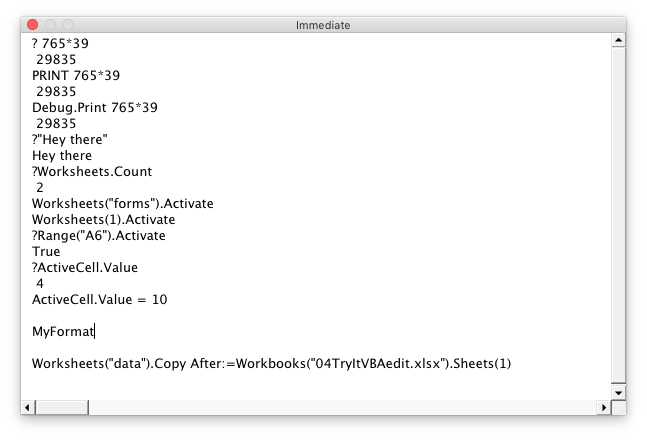
\includegraphics[width=0.8\textwidth]{img/immediate}$$
%%Again, not available for Mac yet, but you can get a pre-release of the new Mac VB Editor using a method found 
%%\href{https://www.youtube.com/watch?v=xHnxjjIeIrQ}{\blue{here (click me)}}
%% NOT TRUE
%\end{frame}




\frame{
\ft{Try It: Immediate Window}
\begin{exampleblock}
{Question:} Try do these actions using the immediate window:
\begin{enumerate}
\item Print {\tt "Hey There!"}
\item Calculate the answer of 765 * 39.
\item Count the number of worksheets.
%\item Select a cell then call the macro bolditalics.
%\item Change the value of cell B4 to "DATA".
%\item Change the value of cell A6 to 100.
\item Switch the active worksheet to \textit{Sheet2}.
\item Switch the active worksheet to \textit{Sheet1} and select cells \cell{A1:A4}.
\item Switch the active cell to \cell{A6} and print its value.
\item Change the value in the current cell ({\tt ActiveCell}) to 10.
\item Use the command {\tt msgbox} to display value in current cell (ActiveCell).
\end{enumerate}
\end{exampleblock}
}




\begin{frame}[fragile]
\ft{Subs}
Most of the macros you write in VBA are Sub procedures.\eol %https://

A \emph{Sub procedure} (also know as a subroutine or ``sub") is set of \textit{commands} to perform a certain task.\eol

In the code window, text is colour coded for ease of readability:
$$\includegraphics[width=0.5\textwidth]{img/subsyntax}$$

\end{frame}



\frame{
\ft{Macro Code in Visual Basic Editor}
The general syntax for a subroutine:
$$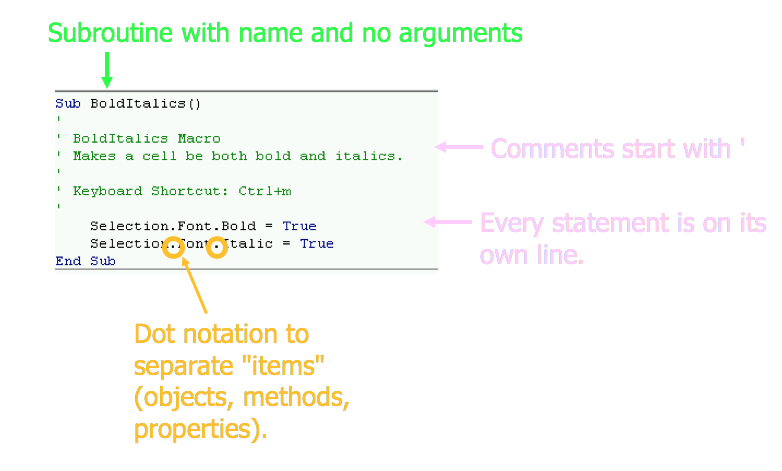
\includegraphics[width=0.99\textwidth]{img/MacroCode}$$
}



\frame{
\ft{{\tt} WITH Statement in Visual Basic Code}
$$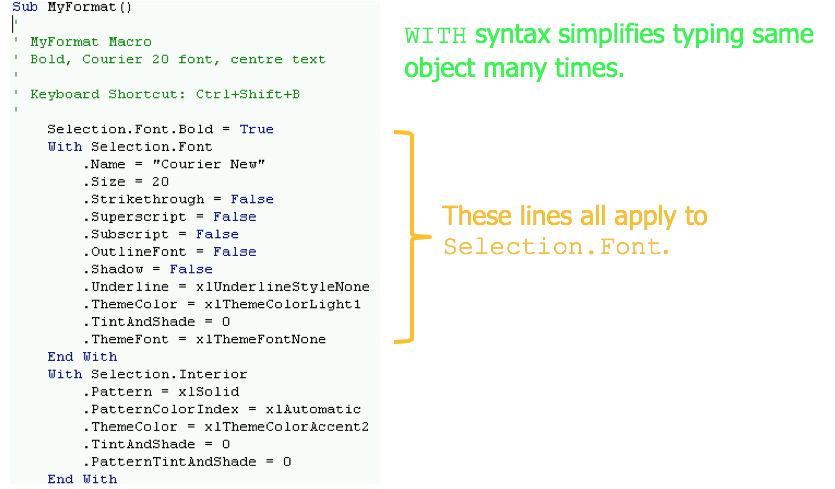
\includegraphics[width=0.99\textwidth]{img/with}$$
}






\begin{frame}
\ft{Advanced: Object-Oriented Programming}
\emph{Object-oriented programming} structures code as objects, classes, methods, and properties.  This organization makes it easier to understand and construct large programs.\eol
An \emph{object} is an instance of a class that has its own properties and methods that define what the object is and what it can do.\eol
A \emph{class} is a generic template (blueprint) for creating an object. \eol
A \emph{property} is an attribute or feature of an object.\eol
A \emph{method} is a set of statements that performs an action.
\end{frame}


%\begin{frame}[fragile]
%\ft{Events}
%An \emph{event} is a notification to your program that something has occurred.\eol
%Events in Excel: 
%\begin{itemize}
%\item add a worksheet
%\item double-click on a cell
%\item change a cell value
%\item calculating a formula
%\item click on a button (can execute a macro)
%\end{itemize}
%Worksheet-level events on a particular worksheet and workbook level events for entire file.
%\end{frame}





\begin{frame}
\ft{Advanced: Object-Oriented Programming}
 All \emph{objects} of a \emph{class} have the \underline{same} \emph{methods} and \emph{properties} (although the property values can be different).\eol
Consider this the analogy: 
 \begin{itemize}
 \item Class: Laptops
\item  Object: MacBookAir
 \item Property: size
 \item Value: MacBookAir.size = 11inch
 \item Method: MacBookAir.PowerOn 
 \end{itemize}
 All laptops will have the same methods that can be performed on them and properties (eg. MicroSoftSurface2.size = 10.6inch,  MicroSoftSurface2.PowerOn)
\end{frame}


%\begin{frame}[fragile]
%\ft{Advanced: Object-Oriented Programming}
%VBA objects that you will encounter include:
%\begin{itemize}
%\item {\tt Application} object, ie. Excel application itself,
%\item  {\tt Workbook} object representing a workbook, 
%\item  {\tt Worksheet} object representing a worksheet, 
%\item {\tt Range}  representing a:
%\begin{itemize}
%\item  individual cell, eg \verb|Range("E5").Select|
%\item range of cells, eg. \verb|Range("A1:C3").Select|
%\item collection of cells, eg \verb|Range("E5,C4,D5").Select|
%\end{itemize}
%\end{itemize}
%\medskip
%Just as variables have data types, Objects have types called classes:\begin{itemize}
%\item eg. Workbook, Worksheet and Range are just a few of Excel's object classes. 
%\end{itemize}
%\medskip
%\textit{What's the difference?:} A class is like a blueprint and consumes no memory.  When you create an ``instance" of this class it becomes an object and consumes memory and can carry out actions. More \href{http://www.cpearson.com/excel/classes.aspx}{here}.
%\end{frame}
%%https://docs.microsoft.com/en-us/dotnet/visual-basic/programming-guide/language-features/objects-and-classes/



\begin{frame}[fragile]
\ft{Advanced: Object-Oriented Programming}
Methods may (or may not) come with extra settings called \emph{arguments/parameters}.  These parameters describe \textit{how} an action is carried out. eg.
\begin{center}
\texttt{MacBookAir.Login  \orange{User:=Irene}}
\end{center}
Consider real VBA code:\\[0.5em]



\blue{\tt Worksheets("data")}.\green{\tt Copy} \orange{\tt  After:=Worksheets("forms")}
\blue{\tt Range("A1")}.\green{\tt Copy}  \orange{\tt Range("A2")} \\
\blue{\tt Application.ActiveDocument}.\green{\tt SaveAs} \orange{\tt ("NewName.docx")}
\blue{\tt ActiveWorkbook}.\green{\tt SaveAs} \orange{\tt ("NewName.xlsm")}
\vfill
\blue{blue} = object,  \green{green} = method, \orange{orange} = argument/parameter
\end{frame}

\begin{frame}[fragile]
\ft{Excel Objects}
Excel structures everything as a hierarchy of objects, and commands are done by running a method of an object.\eol
An object may contain other objects as well as methods and properties. (eg. {\tt ActiveCell} and {\tt ActiveCell.Font} are both objects)\eol
A dot {\tt "."} is used as a separator between objects and subobjects, methods, and properties.\eol
Examples:
\begin{itemize}
 \item {\tt Application} (Top-level object)
\item {\tt Workbook} -- individual Excel file
\item {\tt Worksheet} - sheet in a workbook
\end{itemize}

{\footnotesize \tt Application.ActiveWorkbook.Worksheets("macro").Range("A1").Value}


\end{frame}


\begin{frame}[fragile]
\ft{Collections}\label{collections}
\begin{itemize}
\item \emph{Collections} are variables that store multiple data items. \eol

\item Data items can either be indexed (selected) by name or number. \begin{itemize}
\item example: {\tt Worksheets("macro")}, {\tt Worksheets(2)}
\end{itemize}
{\tt Worksheets} is a collection as there may be multiple worksheets in the workbook.  \eol

\item Collections are indexed starting with 1.\eol
\item Another example is 'Rows' which is a collection object containing all the rows of a Worksheet.
$$ {\tt Worksheets("Sheet1").Rows(3).Delete} $$

\end{itemize}

\end{frame}

\begin{frame}
\ft{Advanced: Object-Oriented Programming}
Building on our first analogy:
 \begin{itemize}
 \item Class: Laptops
\item  Object: MacBookAir
\begin{itemize}
\item {\tt MacBookAir}
\end{itemize}

\item  Sub-object: hard drive, 
\begin{itemize}
\item  {\tt MacBookAir.harddrive}
\end{itemize}

 \item Property: size
 \item Values for example:
 \begin{itemize}
\item {\tt Laptops.MacBookAir.size=10in}
\item {\tt Laptops.MacBookAir.harddrive.size = 500GB}
 \end{itemize}
 \item Method (action): 
 \begin{itemize}
 \item {\tt MacBookAir.Login }
 \end{itemize}

 \end{itemize}
All objects of class {\tt Laptop} should follow the same template.  For example, the should all have a {\tt size} property, a {\tt harddrive} sub-object, etc.
% The class would determine what properties we should expect with this object.  For example if we were talking about weather class, perhaps we would expect objects like {\tt Day}, {\tt Raining}, etc. and calling something like {\tt May20.size} wouldn't make sense.
\end{frame}



\begin{frame}[fragile]
\ft{Advanced: Object-Oriented Programming}
Now lets consider actual VBA code:
 \begin{itemize}
\item  Class: Range
\item  Object: \verb|ActiveCell|,  \verb|Range("A1")|
\item  Sub-object: \verb|ActiveCell.Font|
 \item Property: \verb|ActiveCell.Font.Name|
 \item Value: \verb|ActiveCell.Font.Name = "Times New Roman"|
 \item Method: \verb|Range("A1").Select|
 \end{itemize}
\end{frame}


\begin{frame}
\ft{Analogy}
Here's an analogy that may help
 \begin{itemize}
%\item  Class: category 
%\begin{itemize}
%\item People 
%\end{itemize}

\item  Object: nouns
\begin{itemize}
\item man
\end{itemize}
 \item Property: adjectives (something that describe the object)
\begin{itemize}
\item eg.  height, usage {\tt man.height}
\end{itemize}
\item Method: verbs (action words)
\begin{itemize}
\item eg.  run, usage {\tt man.run}
\end{itemize}
\item Arguments/parameters: adverbs \\
\begin{itemize}
\item eg. quickly, usage {\tt man.run quickly}
\end{itemize}
 \end{itemize}
 \vfill
 While this doesn't fit in with the Grammar analogy, \dots
 \begin{itemize}
  \item \textcolor{gray}{Class}: \textcolor{gray}{Mammals} 
  \item \textcolor{gray}{Value}: \textcolor{gray}{eg.  usage {\tt man.height = "5 foot 11"}}
 \end{itemize}

\end{frame}


%
%\begin{frame}{Object Browser}
%\begin{itemize}
%\item You can access the \emph{Object Browser} by selecting the 
\includegraphics[width=1em]{img/objbrowser.png}\ button on the Toolbar or typing \keystroke{F2}(windows) while in VBA mode or using {\bf View} \ra {\bf Object Browser} from the menu.
%\medskip
%\item Here you can browse through all available objects in your project and see their properties, methods and events. 
%\medskip
%\item In addition, there is an IntelliSense (ie a code-completion) feature while writing VB code:
%\begin{center}
%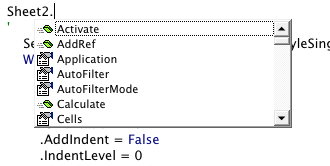
\includegraphics[width=0.6\textwidth]{img/autocomplete.png}
%\end{center}
%\end{itemize}
%\end{frame}
%
%
%%\frame{
%%\ft{Object Browser}
%%$$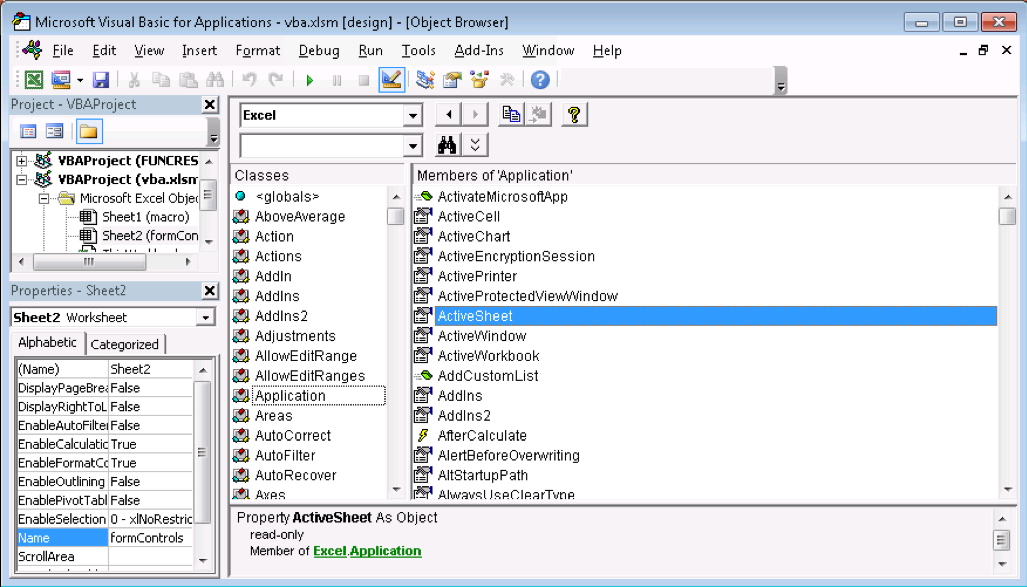
\includegraphics[width=0.9\textwidth]{img/ObjectBrowser}$$
%%}
%%
%
%
%\frame{
%\ft{Object Browser}
%For example, the following methods (as indicated by the 
\includegraphics[width=1em]{img/methods} icon) and properties (as indicated by the 
\includegraphics[width=1em]{img/property} icon) can be applied to the {\tt Range} object:
%$$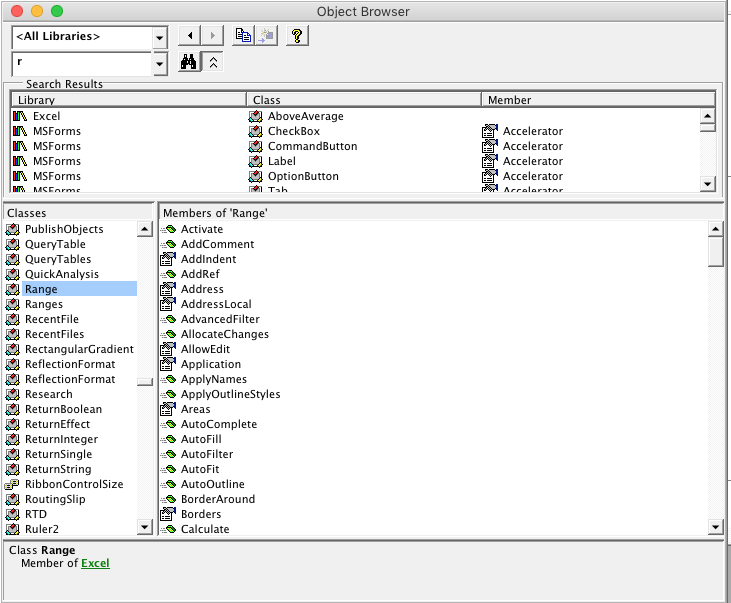
\includegraphics[width=0.9\textwidth]{img/range}$$
%}


%\begin{frame}[fragile]
%\ft{Excel Objects}
%\begin{description}
%\item[Range Object] The {\tt Range} object selects a cell or group of cells.
%Example:
%\begin{itemize}
%\item {\tt Worksheets("Sheet1")}\\
% {\tt \orange{.Range("A1:C3")}.Font.Italic = True}\eol
%\end{itemize}
%
%\item[Object Methods] Methods perform an action.\\
%Example:
%\begin{itemize}
%\item {\tt Worksheets("macro").Activate}
%\end{itemize}
%\end{description}
%%The Workbook object has the methods 'Activate', 'Close', 'Save', \dots
%\end{frame}








\begin{frame}
\begin{example}
How many of the following statements are TRUE?
\begin{itemize}
\item A macro can be created without assigning it a shortcut key.
\item A macro will record cursor movements.
%\item Macros can be created in an individual workbook or in a personal macro workbook so they can be used in multiple workbooks.
\item Macros saved in your Personal Macro Workbook can only be used in the a single workbook.
%\item A macro can have only one command it executes.
\end{itemize}
\begin{multicols}{4}
\begin{enumerate}[A)]
\item 0 
\item 1
\item 2
\item 3
%\item 4
\end{enumerate}
\end{multicols}
\end{example}
\end{frame}


\begin{frame}<handout:0>
\begin{block}{Answer}
How many of the following statements are TRUE?
\begin{itemize}
\item {\color<1->{ForestGreen}{A macro can be created without assigning it a shortcut key.}}
\item {\color<2->{red}{A macro will record cursor movements.}}
\item {\color<3->{red}{ Macros saved in your Personal Macro Workbook can only be used in the a single workbook.}}
%\item {\color<4->{ForestGreen}{A macro can have only one command it executes.}}
\end{itemize}
\begin{multicols}{4}
\begin{enumerate}[A)]
\item 0 
\item \textbf<4>{\textit<4>{{\color<4>{iyellow}{1}}}}
\item 2
\item 3
%\item 4
\end{enumerate}
\end{multicols}
\end{block}
\end{frame}



\begin{frame}
\begin{example}
How many of the following statements are TRUE?
\begin{enumerate}
\item A method can have no parameters.
%\item Two objects of the same class have the same properties.
\item Two objects of the same class will have the same values for any given property.
\item Workbook is the top-level object in Excel.
\end{enumerate}
\begin{multicols}{4}
\begin{enumerate}[A)]
\item 0 
\item 1
\item 2
\item 3
\end{enumerate}
\end{multicols}
\end{example}
\end{frame}



\begin{frame}<handout:0>
\begin{block}{Answer}
How many of the following statements are TRUE?
\begin{enumerate}
\item {\color<1->{ForestGreen}{A method can have no parameters.}}
%\item {\color<2->{ForestGreen}{Two objects of the same class have the same properties.}}
\item {\color<3->{red}{Two objects of the same class will have the same values for any given property.}}
\item {\color<4->{red}{Workbook is the top-level object in Excel.}}
\end{enumerate}
\begin{multicols}{4}
\begin{enumerate}[A)]
\item 0 
\item \textbf<4>{\textit<4>{{\color<4>{iyellow}{1}}}}
\item 2
\item 3

\end{enumerate}
\end{multicols}
\end{block}
\end{frame}





\frame{
\ft{Challenge Try it: Create a Macro in VBE}
\begin{exampleblock}
{Question} Copy the {\tt MyFormat} macro and edit to produce a new macro called {\tt RedUnderline} that:
\begin{itemize}
\item Convert to plain text; that is, if the cell was bold or italics before, resets to not have bold or italics.
\item Underlines the text in the cell.
\item Makes the cell background red.
\end{itemize}

\end{exampleblock}
See hints on next page
} 

\frame{
\ft{Challenge Try it: Create a Macro in VBE}
Hints:
\begin{itemize}
\item Underline property in Excel is {\tt Font.Underline} and can set to constant {\tt xlUnderlineStyleSingle}.
\medskip
\item Can change background colour with {\tt Interior.Color} and set to {\tt RGB(redValue, greenValue, blueValue)} where the colour values are numbers from 0 to 255.  See more on this \href{https://access-excel.tips/excel-vba-color-code-list/}{here}.
\medskip
\item Alternatively you could use the ColorIndex values.  See more \href{http://dmcritchie.mvps.org/excel/colors.htm}{here}
\medskip
\end{itemize}
}


\begin{frame}{}

\begin{exampleblock}
{Exercise:}  Assign the {\tt MyFormat} and {\tt RedUnderline} macro to a single subroutine called {\tt Button2\_Click}.  Assign this new macro to a button in your excel file.
\end{exampleblock}

{\bf Hint:} Within VBA, you can call macros by name.  %For example, lets assign multiple macros to a single button.  
See instructions on the next page.
\end{frame}

\begin{frame}[fragile]
\ft{Macro Buttons}
\begin{enumerate}
\item Select the {\bf Developer} tab and click 
$$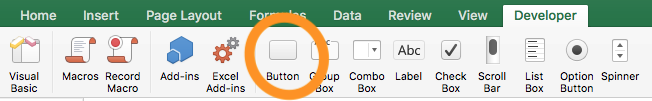
\includegraphics[height=3.5em]{img/button.png}.$$
\item To prompt the Assign Macro popup window, click where you would like this button to appear on your worksheet.
\item Select {\bf New} to open the VBA editor and Type the name of the macros you wish to assign in the body of the Sub.
\begin{verbatim}
  Sub ButtonClick() 
      MyFormat
      RedUnderline
  End Sub
\end{verbatim}
\end{enumerate}
\end{frame}



\section{UDF}
\frame{
{\Large Creating Excel Functions}

As mentioned previously, recording macros are restrictive in that they can't performs loops.\eol

If we want to loop a procedure we can/need to code it up ourselves.\eol

In addition, we will learn how we can create our own \emph{functions} which we refer to as User Defined Functions (UDF)
\eol
But first things first, \dots
\eol

}


\frame{
\ft{Introduction to Programing}
An \emph{algorithm} is a precise sequence of steps to produce a result.  A program is an encoding of an algorithm in a \emph{language} to solve a particular problem.\eol

There are numerous languages that programmers can use to specify instructions.  Each language has its different features, benefits, and usefulness.\eol

We will start with Excel VBA but also study Python and R.\eol

The goal is to understand fundamental programming concepts that apply to all languages.
}

\begin{frame}[fragile]
\frametitle{Variables}
A \emph{variable} is a name that refers to a location that stores a data value.
$$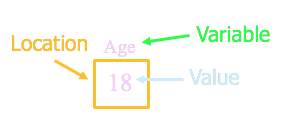
\includegraphics[width=0.4\textwidth]{img/Variable}$$
\begin{alert}
{IMPORTANT:} The \emph{value} at a location can change using initialization or assignment.\eol
\end{alert}
\emph{Assignment} using an  sets the value of a variable.\eol
Example:
\begin{itemize}
\item 
\begin{verbatim}
num = 10
num = Range("A1").Value
\end{verbatim}
\end{itemize}
\end{frame}

\begin{frame}[fragile]
\ft{Excel Variables}
Variables increase code efficiency and readability.\eol
Every variable in Excel has a \emph{name} and a \emph{data type}.\eol
Data types include: Boolean (TRUE or FALSE), Currency, Date, Double, Integer, Long, Object, String, Variant (any type)%; see more on data types \href{http://www.informit.com/articles/article.aspx?p=339929&seqNum=2}{here}.
\begin{itemize}
\item See Part 2 of \href{https://www.excelfunctions.net/excel-vba-tutorial.html}{\blue{this (click me)}} tutorial for more on this.
\end{itemize}


Example:
\begin{itemize}
\item[] 
{\tt \yellow{Dim} num \yellow{As Integer}}\eol
\end{itemize}
The {\tt \yellow{Dim}} keyword \emph{declares} the variable (named {\tt num}) as an integer.\eol
{\bf Sidenote:} A declaration may be optional or required, depending on the programming language.

\end{frame}
% https://www.excelfunctions.net/vba-variables-and-constants.html
%From the above table, it is clear that you can save on memory by using specific data types (e.g. Integers rather than Longs, or Singles rather than Doubles). However, if you are planning to use the 'smaller' data types, you must be sure that your code will not encounter larger values than can be handled by the chosen data type.


\begin{frame}
\ft{Excel Variables}
There are number of different declaration keywords we can use. for example:
\begin{description}
\item[Const] for setting constants
\item[Static] for setting constants
\item[Public] for using across macros (default declaration for subs)
\item[Private] variable is limited to the current module
\item[Public Const] for setting constants across macros
\item[\dots]
%\item[Set] \dots)
\end{description}
 % Set for objects to a variable: https://www.excelfunctions.net/excel-objects.html
%There are also different variable types (eg. Boolean, Single, Double, String, Variant, \dots) \eol
\medskip
For example, to declare a constant in VBA:\\
\begin{itemize}
\item[] {\tt \yellow{Const} MaxCount = 5000}
\end{itemize}
\end{frame}


% declaring strings: https://docs.microsoft.com/en-us/dotnet/visual-basic/programming-guide/language-features/strings/string-basics
\begin{frame}
\ft{Excel Variables - Strings}
We can also declare \emph{strings} i.e. a series of characters.% (or {\tt Char} type variables)
\medskip
\begin{itemize}
\item[] {\tt \yellow{Dim}  MyString  \yellow{As String}}
\item[] {\tt MyString = "This is an example of the String"}
\end{itemize}
We can declare and assign strings all in one step:
\begin{itemize}
\item[] {\tt \yellow{Dim}  MyString  \yellow{As String} = "ABCDE"}
\end{itemize}
\medskip
Notice that a {\tt Char}  type is restricted to be a single character.  For example:
\begin{itemize}
\item[] {\tt \yellow{Dim}  MyString  \yellow{As String} = "ABCDE"}
\item[] {\tt \yellow{Dim}  myChar  \yellow{Char}}
\item[] {\tt \green{' The value of myChar is "D".}}
\item[] {\tt myChar = myString.Chars(3)}
\end{itemize}
See more about this topic \href{https://docs.microsoft.com/en-us/dotnet/visual-basic/programming-guide/language-features/strings/string-basics}{here}.
\end{frame}


\begin{frame}
\ft{Excel Variables - Arrays}
We can also define \emph{arrays} which are data structure consisting of a collection of elements (values or variables).\eol

Each element is identified by an \textit{index} or \textit{key}.\eol
\begin{figure}[htbp]
\begin{center}
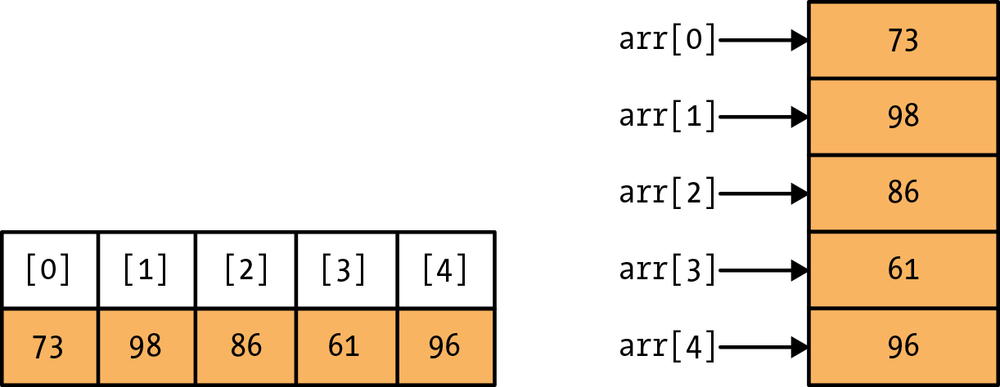
\includegraphics[width=0.67\textwidth]{img/array.png}
\caption{Source: \href{https://www.oreilly.com/library/view/computer-science-programming/9781449356835/sixdot2_array_types.html}{O'Reilly Media}}
\label{default}
\end{center}
\end{figure}
\begin{alertblock}{}
\red{\bf Warning:} Depending on the programming language, sometimes this index will begin from 0, other times it will begin from 1 (in VBA we are able choose either). 
\end{alertblock}

\end{frame}

\begin{frame}
\ft{Excel Variables - Arrays}
\emph{Arrays} are declared the same way as other variables, the only difference is that now, we need to specify its length.\eol
By default, arrays are indexed starting from 0. Hence 
$${\tt \yellow{Dim}\ Class\_List\blue{(150)} \ \yellow{As\ String}}$$
 would be recognized as an array of 150 variables, which are indexed from 0 to 149.
  \begin{itemize}
\item[] 
{\tt Class\_List(0) = "Irene Vrbik"}\\
{\tt Class\_List(1) = "Peter Gregory"}
\end{itemize}
If you want your index to start from 1 rather than 0, use:
\begin{itemize}
\item[] 
{\tt \yellow{Dim}  MidtermGrades \blue{(1 To 150)} \yellow{As Integer}}  \\
{\tt MidtermGrades(1) =  89}\\
{\tt MidtermGrades(2) = 91}
\end{itemize}
%The {\tt \blue{(1 To 150)}} tells Excel that {\tt Class\_List} in an array of 150 String variables.\eol
For more on this subject click \href{https://powerspreadsheets.com/excel-vba-array/}{here}.
\end{frame}

\begin{frame}{Option Explicit Option}
Although VBA does not require us to declare variables, it is good coding practice to do so.\eol%\footnote{force explicit declaration with ``Option Explicit" at the top of your file} \eol
By default, all undeclared variable in Excel will have the Variant type (which can hold Dates, Floating Point Numbers or Strings of Characters)\eol
If you want to prevent default declarations, you can always set the ``Option Explicit" option for force you to explicitly declare each variable. Read more about it \href{https://www.excelfunctions.net/vba-variables-and-constants.html}{here}.

\end{frame}



\begin{frame}[fragile]
\ft{Variables Question}
\begin{exampleblock}
{Question} How many of the following statements are TRUE?
\begin{enumerate}
\item A variable name cannot change during a program.
\item A variable value cannot change during a program.
\item A collection is a variable that can store multiple data items.
\end{enumerate}
\begin{multicols}{4}
\begin{enumerate}[A)]
\item 0 
\item 1
\item 2
\item 3
\end{enumerate}
\end{multicols}
\end{exampleblock}
\end{frame}


\begin{frame}<handout:0>[fragile]
\ft{Variables Question}
\begin{block}
{Question} How many of the following statements are TRUE?
\begin{enumerate}
\item {\color<1->{sgreen}{A variable name cannot change during a program.}}
\item {\color<2->{red}{A variable value cannot change during a program.}}
\item {\color<3->{sgreen}{A collection is a variable that can store multiple data items.}}
\end{enumerate}
\begin{multicols}{4}
\begin{enumerate}[A)]
\item 0 
\item 1
\item \textbf<4>{\textit<4>{{\color<4>{iyellow}{2}}}}
\item 3
\end{enumerate}
\end{multicols}
\end{block}
\end{frame}

\begin{frame}[fragile]
\ft{Variables Question}
\begin{exampleblock}
{Question} How many of the following statements are TRUE?
\begin{enumerate}
\item A value in a collection can be retrieved by name or by index starting from 0.
\item In Excel, variables can be  declared using {\tt Dim}.
\item In Excel, variables are declared with a data type.
\end{enumerate}
\begin{multicols}{4}
\begin{enumerate}[A)]
\item 0 
\item 1
\item 2
\item 3
\end{enumerate}
\end{multicols}
\end{exampleblock}
\end{frame}


\begin{frame}<handout:0>[fragile]
\ft{Variables Question}
\begin{block}
{Question} How many of the following statements are TRUE?
\begin{enumerate}
\item {\color<1->{red}{A value in a collection can be retrieved by name or by index starting from 0.}}
\item {\color<2->{sgreen}{In Excel, variables can be  declared using {\tt Dim}.}}
\item {\color<3->{sgreen}{In Excel, variables are declared with a data type.}}
\end{enumerate}
\begin{multicols}{4}
\begin{enumerate}[A)]
\item 0 
\item 1
\item \textbf<4>{\textit<4>{{\color<4>{iyellow}{2}}}}
\item 3
\end{enumerate}
\end{multicols}
\end{block}
\end{frame}



\begin{frame}[fragile]
\ft{Decisions}
Decisions allow the program to perform different actions in certain conditions. \eol
Logical operators: {\tt AND, OR, NOT}\eol
Example decision syntax:
\begin{itemize}
\item 
\begin{verbatim}
If condition Then
    statement
End If
\end{verbatim}
\end{itemize}
\begin{itemize}
\item 
\begin{verbatim}
If condition Then
    statement if true
Else
    statement if false
End If
\end{verbatim}
\end{itemize}
\end{frame}

\begin{frame}[fragile]
\ft{Question: Decisions}
\begin{example}
 What is the output of the following code:
$$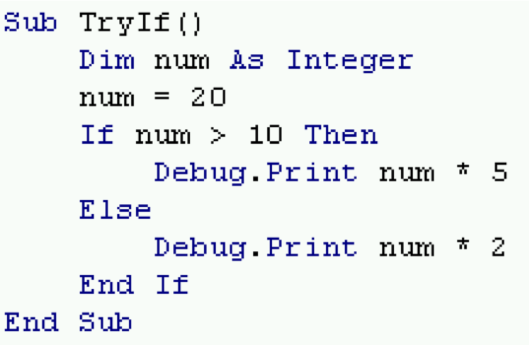
\includegraphics[width=0.4\textwidth]{img/Qcode}$$
\begin{multicols}{4}
\begin{enumerate}[A)]
\item 100
\item 40
\item 20
\item error
\end{enumerate}
\end{multicols}
\end{example}
\end{frame}

\begin{frame}[fragile]
We can verify this result by running the {\tt TryIf} sub found in the {\bf 04VBA.xlsm} file.
\medskip
To step through you code in , navigate to the {\tt TryIf()} function and press \keystroke{F8} on a windows or press this button:
$$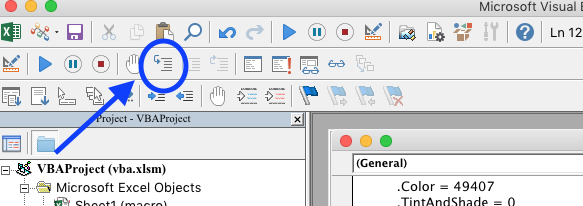
\includegraphics[width=0.6\textwidth]{img/step.png}$$
\medskip
Alternatively you could type
\begin{Verbatim}[frame=single]
TryIf
\end{Verbatim}
into the Immediate window and press \keystroke{ENTER}.
\end{frame}



\begin{frame}<handout:0>[fragile]
\ft{Question: Decisions}
\begin{block}
{Question} What is the output of the following code:
$$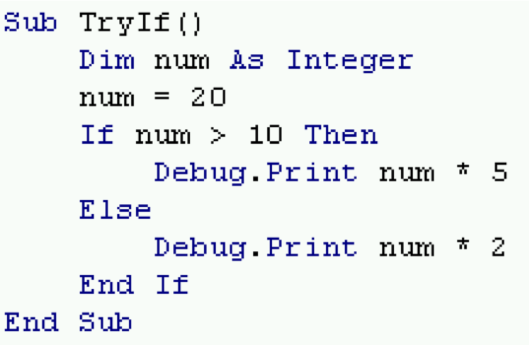
\includegraphics[width=0.4\textwidth]{img/Qcode}$$
\begin{multicols}{4}
\begin{enumerate}[A)]
\item \textbf<1>{\textit<1>{{\color<1>{iyellow}{100}}}}
\item 40
\item 20
\item error
\end{enumerate}
\end{multicols}
\end{block}
\end{frame}

\begin{frame}[t,fragile]
\ft{Try It: Decisions}
\begin{exampleblock}
{Question} Create a method called {\tt EchoDecision} that asks user a Yes and No question and outputs a message either {\tt "Yes"} or {\tt "No"} depending on what they chose.
\end{exampleblock} 
$$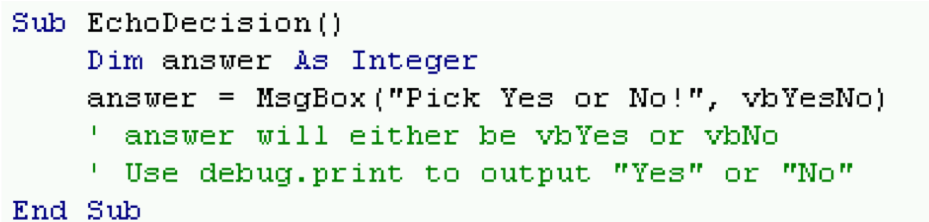
\includegraphics[width=0.9\textwidth]{img/trydecide}$$
MsgBox function in VBA displays a message in a window and waits for click on a button.\eol
Debug.Print is telling VBA to print that information in the Immediate Window.  
\end{frame}





\begin{frame}[fragile]
\ft{Loops and Iteration}
A \emph{loop} repeats a set of statements multiple times until some condition is satisfied.\eol
Each time a loop is executed is called an \emph{iteration}.\eol
A \emph{{\tt for} loop} repeats statements a given number of times.

Example:
\begin{itemize}
\item 
\begin{verbatim}
Dim i As Integer
For i = 1 To 5
    Debug.Print i
Next i
\end{verbatim}
\end{itemize}
The above will print out the numbers 1 to 5 \textit{\alert{inclusively}}. 
\end{frame}

\begin{frame}[fragile]
\ft{Question: loops}
\begin{exampleblock}
{Question} How many numbers are printed with this loop?
$$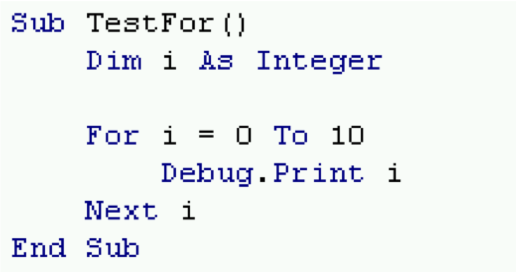
\includegraphics[width=0.4\textwidth]{img/printedloop}$$
\begin{multicols}{4}
\begin{enumerate}[A)]
\item 11
\item 10
\item 0
\item error
\end{enumerate}
\end{multicols}
\end{exampleblock}
\end{frame}


\begin{frame}<handout:0>[fragile]
\ft{Question: loops}
\begin{block}
{Question} How many numbers are printed with this loop?
$$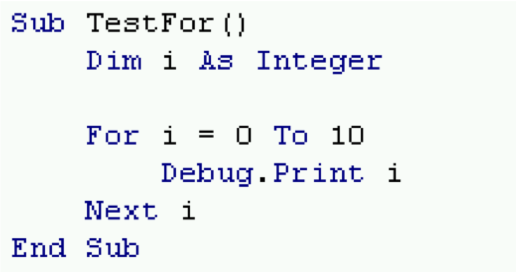
\includegraphics[width=0.4\textwidth]{img/printedloop}$$
\begin{multicols}{4}
\begin{enumerate}[A)]
\item \textbf<1>{\textit<1>{{\color<1>{iyellow}{11}}}}
\item 10
\item 0
\item error
\end{enumerate}
\end{multicols}
\end{block}
\end{frame}
%
%\begin{frame}[fragile]
%\ft{Try it: loops}
%\begin{exampleblock}
%{Homework:} Create a method called {\tt TryFor} that prints the numbers 1 to 10. \\[1em]
% Challenging variants:
%\begin{enumerate}[a)]
%\item Print the numbers from 10 down to 1.
%\item Print only the even numbers from 1 to 10.
%\end{enumerate}
%\end{exampleblock}
%{\bf Hint:} use the \href{https://www.excel-easy.com/vba/examples/step-keyword.html}{\tt Step} keyword to specify a different increment for the counter variable of a loop.
%\end{frame}

\begin{frame}[fragile]
\ft{UDF General Syntax}
A user-defined function is your own Excel function that can be used in cell formulas like built-in functions.\eol

A UDF must return a number, string, array, or Boolean.  We declare the data type of the returned value directly after any argument.\eol

Notice the data types of each argument using the {\tt As} keyword. \eol
The general syntax for creating a UDF is:\\
\verb|Function FunctionName(arg1 As DataType, ...) As DataType|\\
\verb|     'comments|\\
\verb|     [Statements]|\\
\verb|End Function|
\end{frame}

\begin{frame}[fragile]{User-Defined Functions (UDFs)}
%\end{frame}
%
%\begin{frame}[fragile]
%\ft{User-Defined Functions (UDFs)}
Example: UDF {\tt doubleIt} will double the input argument.
$$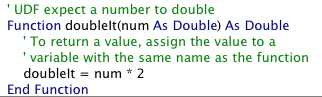
\includegraphics[width=0.6\textwidth]{img/UDF.png}$$
\alert{N.B} The value returned must be assigned to a variable with the same name as the UDF (this variable is implicitly declared in the first line).
\begin{itemize}
\item That is, {\tt doubleIt} stores the value returned by our function {\tt doubleIt}.
\item N.B. If the function data type is not declared, it is assumed to be {\tt Variant}
\end{itemize}

\end{frame}


\begin{frame}
\ft{Sub vs. UDFs}
%A Sub procedure (also know as a subroutine) is set of commands to perform a certain task.\eol

Unlike a Sub, a UDF cannot change the Excel environment including the current cells or other cells (e.g. change formatting). \eol

Unlike a UDF, a Sub procedure does not return a result, nor can they be typed directly into a Worksheet in Excel
\begin{itemize}
\item eg. the function SUM() returns a result of summing a group of numbers
\item the Sub might carry out actions like formatting a set of cells\eol
\end{itemize}
Most of the macros you write in VBA are Sub procedures.\eol %https://powerspreadsheets.com/vba-sub-procedures/
Both VBA Sub procedures and UDF procedures can take arguments but they are not essential.
\end{frame}





\begin{frame}
\ft{UDF Example: Sum Cells by Background Colour}
The function {\tt SumColor} works like the {\tt SUM()} function, only now, it will only consider the cells having a certain background colour. \eol
This function takes two arguments. 
\begin{enumerate}
\item  The first specifies where in the table are we looking for values to add (i.e. a range of cells).  \item The second argument specifies the background colour.
\end{enumerate}
\medskip
Colours can be index by integers.  See \href{http://dmcritchie.mvps.org/excel/colors.htm}{\blue{this}} reference for   for more on colour indexing. For example:
\begin{itemize}
\item Black = 1, White = 2, Red = 3, \dots, Yellowy Orange = 44, Light Orange = 45, Another Orange = 46
\end{itemize}

\end{frame}

\begin{frame}
$$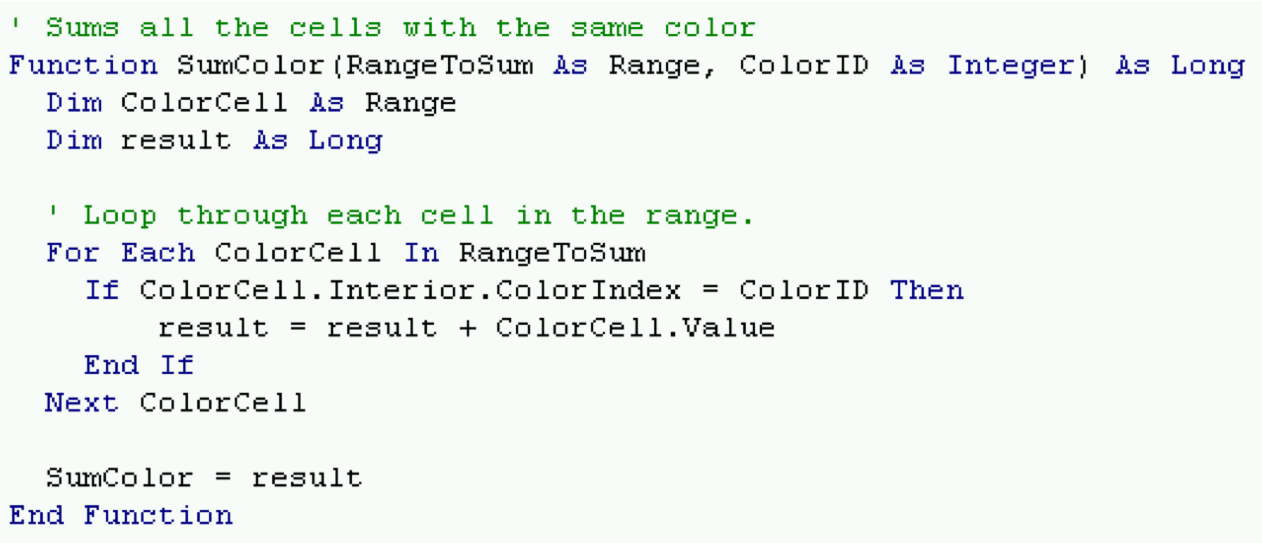
\includegraphics[width=0.99\textwidth]{img/UDFsum}$$
\end{frame}


\begin{frame}
Let's use the function {\tt SumColor} to find the sum of all the cells that have been formatted in orange by the macro {\tt MyFormat}.  \eol
We will need to know the colour index for the colour used in this macro for the input for {\tt ColorID}.\eol
To obtain that, we can either go to the VBA code, go to the colour indexing \href{http://dmcritchie.mvps.org/excel/colors.htm}{link} and look for orange (which might be hard to distinguish by eye), or obtain it from the Immediate Window by typing 
$${\tt ?Range("A6").Interior.ColorIndex}$$
assuming cell \cell{A6} has been formatted using {\tt MyFormat}.\eol
\end{frame}

\begin{frame}
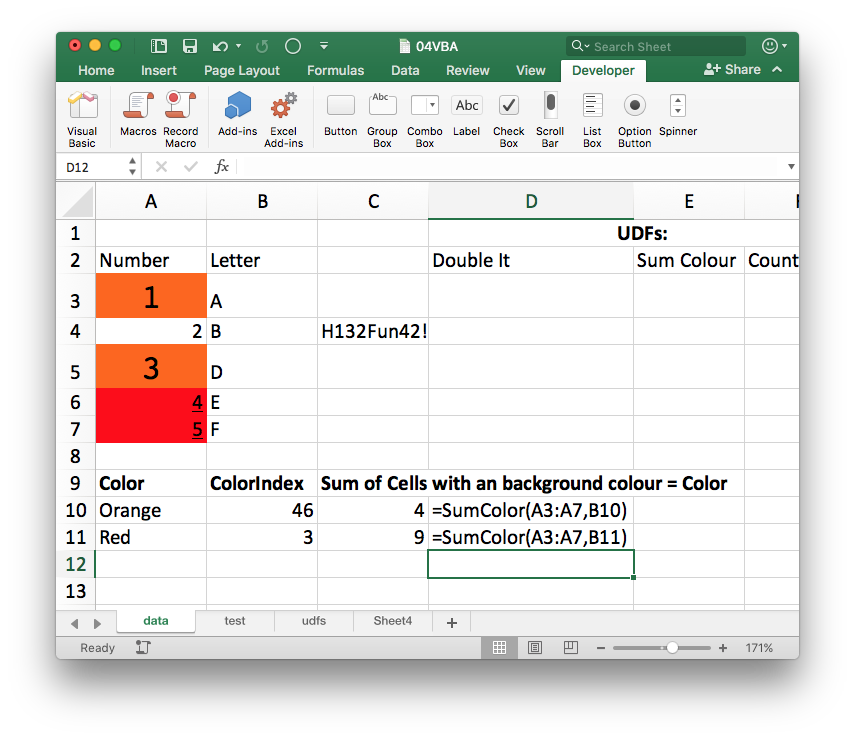
\includegraphics[width=0.9\textwidth]{img/sumcolorsol.png}
\end{frame}


\begin{frame}
\begin{exampleblock}
{Question:}  Create a UDF called {\tt CountNumbers} that will return a count of the number of digits (ie 0 to 9) in a string.  eg. applying this function to the string {\tt Data301} should return 3 (since this course code contains 3 numbers).
\end{exampleblock}
To build this function use:
\begin{itemize}
\item \href{https://exceljet.net/excel-functions/excel-len-function}{\tt Len()} to count the length of the string, and
\item \href{https://exceljet.net/excel-functions/excel-mid-function}{\tt Mid()} to extract  a given number of characters from the middle of a supplied text string. For example, {\tt =MID("apple",2,3)} returns "ppl" (start at index 2, extract a sting of length 3).
%\item \href{https://exceljet.net/excel-functions/excel-isnumber-function}{\tt IsNumber()} to check if the character is a number or not
\item \href{https://www.techonthenet.com/excel/formulas/isnumeric.php}{\tt IsNumeric()} is a VBA function that returns TRUE if the expression is a valid number.
\end{itemize}
\end{frame}

\begin{frame}{VBA functions vs Excel Functions}
\begin{itemize}
\item VBA functions can be used in any program that supports VBA (including Microsoft Word and Access). List of them \href{https://www.excelfunctions.net/vba-functions.html}{here}.\medskip
\item Worksheet functions are specific to Excel and can be used using {\tt Application.WorksheetFunction.[function name]} in VBA code or simply by calling them by name (with any necessary arguments) in a cell, eg. {\tt MID("example", 1, 2)}
\medskip
\end{itemize}
 Read more about the differences between VBA functions and Excel Functions \href{https://spreadsheeto.com/vba-vlookup/}{here}.  Note that:
\medskip
\begin{itemize}
\item  \href{https://exceljet.net/excel-functions/excel-isnumber-function}{\tt IsNumber()} is a worksheet function to check if a value is \textit{stored} as a number, whereas IsNumeric checks is a value can be \textit{converted} to a number.
\item \href{https://www.techonthenet.com/excel/formulas/mid.php}{\tt Mid()} and \href{https://www.techonthenet.com/excel/formulas/len.php}{\tt len()} are both Worksheet functions (WS) \textit{and}
VBA functions (VBA) %https://www.ozgrid.com/forum/forum/help-forums/excel-general/28049-difference-between-isnumeric-and-isnumber
\end{itemize}

\end{frame}



\begin{frame}
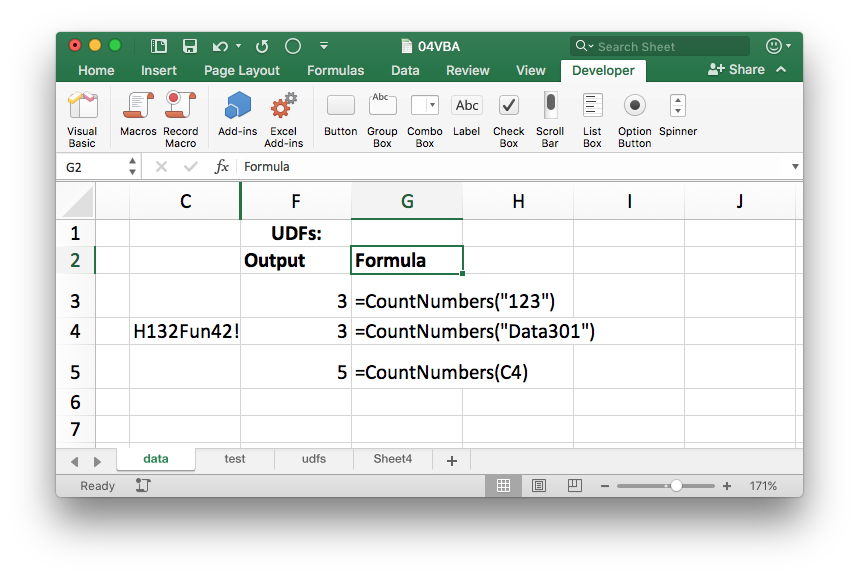
\includegraphics[width=0.9\textwidth]{img/CountNumbersSol}
\end{frame}





%\begin{frame}[fragile]
%\ft{Forms and Input Controls}
%Excel allows the creation of forms with controls for a better interface.\eol
%
%There are two types of controls in Excel:
%\begin{enumerate}
%\item Form controls -- default
%\item ActiveX controls -- allow more flexibility and customization\eol
%\end{enumerate}
%
%Controls can be inserted from the Developer tab. 
%\begin{itemize}
%\item Select {\bf Insert}, pick control (eg. {\bf check box, textbox}), and then click and drag the size and shape of the control on the spreadsheet.
%\end{itemize}
%\end{frame}
%
%\begin{frame}
%You can limit user entries by forcing users to choose a value from a drop-down list.\eol
%To create one, we use the {\bf  Data Validation} feature using the following steps:
%\begin{enumerate}
%\item Store the desired options in a range of cells\label{step1}
%\item Select the cell(s) where you would like your drop-down menu to appear.
%\item Navigate to the \underline{menu} bar (not ribbon) and go to {\bf Data} $>$ {\bf Validation}
%\item Select  ``List" from the {\bf Allow} option's drop-down list. 
%\item Select the cells from step \ref{step1}. as our {\bf Source}
%\end{enumerate}
%N.B. You can only see the drop-down if you click on the cell.
%\end{frame}
%
%\begin{frame}
%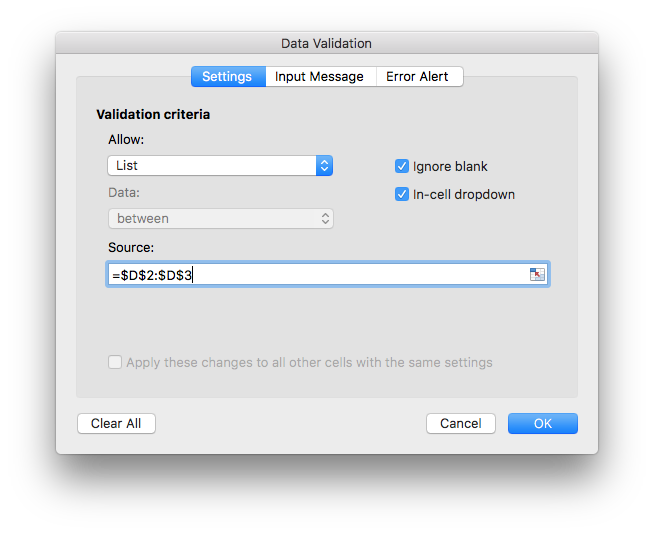
\includegraphics[width=0.9\textwidth]{img/dataval}
%\end{frame}
%
%
%\begin{frame}[fragile]
%\ft{Input Controls}
%$$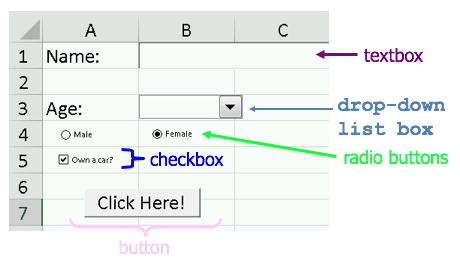
\includegraphics[width=0.8\textwidth]{img/InputControls.png}$$
%\end{frame}

\begin{frame}[fragile]
\ft{Conclusion}
\emph{Microsoft Excel VBA} allows for automating tasks in Excel and provides a full programming environment for data analysis.\eol

\emph{Macros} record a set of actions so they can be easily executed again. \alert{Be aware of security risks when using macros.}\eol

The \emph{Visual Basic Editor (VBE)} is a complete integrated development environment for editing macros and \emph{user-defined functions}.% and adding %forms and 
controls that dynamically respond to events.\eol

Excel VBA uses \emph{object-oriented programming} that structures code as object, classes, methods, and properties.  A developer can control and automate everything with Excel using VBA.
\end{frame}

\begin{frame}[fragile]
\ft{Objectives}
\begin{itemize}
\item List some reasons to use Excel VBA
\item Define macro and explain the benefit of using macros
\item Be able to record and execute a macro
\item Explain the security issues with macros and how Excel deals with them
\item List and explain the use of the four main windows of the Visual Basic Editor
\item Explain the role of the object browser
\item Explain and use the WITH statement syntax
\item Be able to write simple macros using the VBE
\item Define: algorithm, program, language
\item Define: object-oriented programming, object, class, property, method
\item Understand and use dot-notation
\item Use the Range object to select a group of cells
\end{itemize}
\end{frame}

\begin{frame}[fragile]
\ft{Objectives (2)}
\begin{itemize}
\item Define: variable, value, location
\item Create and use Excel variables
\item Explain how a collection is different from a typical variable
\item Use If/Then/Else syntax to make decisions
\item Use For loop for repetition
\item Create user-defined functions and use them in formulas
%\item Define: event
\item List some typical user interface controls
\item Understand that Excel allows for forms and controls to be added to a worksheet which respond to events
\end{itemize}
\end{frame}


%\begin{frame}[label=current]
%  {Questions}
%
%  \nocite{lorem,ipsum}
%  \bibliographystyle{plain}
%  \bibliography{../demo}
%
%\end{frame}

\end{document}

